
\section{Newton Polynomial Interpolation}
\subsection{Collocation}
Collocation = All data points are hit by the approximating function (e.g., polynomial).
The polynomial
\[y(x) = p(x) = c_0 + c_1x^1 + c_2x^2 + \ldots + c_mx^m \qquad \text{with} \quad y(x_k)=p(x_k)=y_k \quad (k=0,1,\ldots,n) \]
results in a linear system of $n+1$ equations.


\subsection{Aitken-Neville Recursion Formula}
Overlapping polynomial interpolation functions
$f_1=p_{0,1,\ldots,n-1}$, $f_2=p_{1,\ldots,n}$ at the data points $x_1,\ldots, x_{n-1}$ can be combined.

\begin{minipage}{8cm}
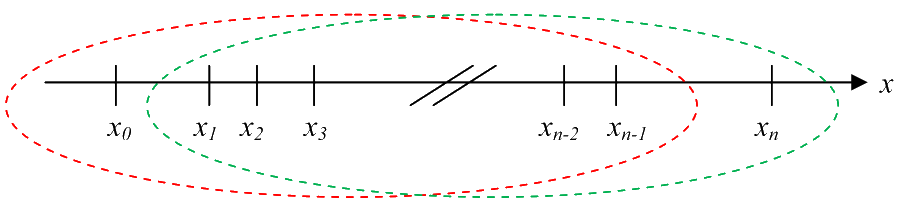
\includegraphics[width=\textwidth]{bilder/aitkenNevilleIdee}
\end{minipage}
\hfill
\begin{minipage}{11cm}
    \[
        p(x) = p_{0,1,\ldots,n}(x) = \frac{(x-x_0) \cdot \overbrace{p_{1,2,\ldots,n}}^{\text{green}}(x) - (x-x_n) \cdot \overbrace{p_{0,1,\ldots,n-1}}^{\text{red}}(x)}{(x_n - x_0)}
    \]
\end{minipage}

\subsection{Newton Polynomials} \label{ssec:newton_polynom}
\textbf{Properties}
\begin{liste}
	\item[\textbf{+}] Embedded (When a data point is added, not everything needs to be recalculated)
	\item[\textbf{+}] A single formula
	\item[\textbf{+}] Practical: Measurements are uniformly distributed.
	\item[$\mathbf{-}$] Runge's phenomenon (Oscillations at the edges)
	\item[$\mathbf{-}$] Computationally expensive
\end{liste}

\begin{minipage}[t]{7.5cm}
	\begin{align}
		y_0 &= a_0\cdot \pi_0 \nonumber\\
		&\quad \downarrow\nonumber\\
		y_1 &= a_0\cdot \pi_0 +a_1\cdot\pi_1 \nonumber\\
		&\quad \downarrow \hspace{1.2cm}\downarrow\nonumber\\
		y_2 &= a_0\cdot \pi_0 +a_1\cdot\pi_1  +a_2\cdot\pi_2  \nonumber\\
		&\vdots\hspace{0.3cm}\downarrow \hspace{1.5cm}\searrow\hspace{1.5cm}\searrow\nonumber\\
		y_n &= a_0\cdot \pi_0(x_n) +a_1\cdot\pi_1(x_n)  +a_2\cdot\pi_2(x_n)+\ldots+ a_n\pi_n(x_n) \nonumber
	\end{align}

	Approximation of a ``measurement data set'' (Messreihe) with polynomials: $$y(x)\approx p(x) = a_0 \pi_0(x) + a_1 \pi_1(x) + \ldots+ a_{n} \pi_{n}(x)$$
\end{minipage}
\hfill
\begin{minipage}[t]{11.5cm}
	\begin{align}
		\pi_0 &= 1 \nonumber\\
		\pi_1 &= (x-x_0) \nonumber\\
		\pi_2 &= (x-x_0)(x-x_1) \nonumber\\
		&\vdots \nonumber\\
		\pi_n &= (x-x_0)(x-x_1)\ldots(x-x_{n-1}) \nonumber\\
		\pi_{n+1} &= (x-x_0)(x-x_1)\cdots(x-x_{n-1})(x-x_n) \nonumber
	\end{align}
\end{minipage}

\subsection{Divided Differences}
Note:
\[
	a_{p-1} = y(x_0,x_1,x_2, ... , x_{p-1}) \text{ belongs to } \pi_{p-1}=(x-x_0)\cdot(x-x_1)\cdot ... \cdot (x-x_{p-2})
\]
More elegant and faster resolution of Newton polynomials.
$$y(x_\mathbf{0}, x_1, \ldots x_\mathbf{k}) = \frac{y(x_\mathbf{1},x_2,\ldots x_\mathbf{k})-y(x_\mathbf{0},x_1,\ldots x_{\mathbf{k-1}})}{(x_k-x_0)} \quad (k=0,1,\ldots,n)$$
$$a(x_\mathbf{0},\ldots,x_\mathbf{n})=\frac{a(x_\mathbf{1},\ldots,x_\mathbf{n})-a(x_\mathbf{0},\ldots,x_{\mathbf{n-1}})}{x_n-x_0}$$
\begin{tabular}{ll}
$k=0$ &$y(x_0)$ \\[0.2cm]
$k=1$ &$\frac{y(x_1)-y(x_0)}{(x_1-x_0)}$\\[0.2cm]
$k=2$ &$\frac{y(x_1,x_2)-y(x_0,x_1)}{(x_2-x_0)}$\\[0.2cm]
$k=3$ &$\frac{y(x_1,x_2,x_3)-y(x_0,x_1,x_2)}{(x_3-x_0)}$\\
\end{tabular}\\
\\

\textbf{Symmetry:} $y(x_0,x_1) = y(x_1,x_0) \Longrightarrow y(x_0,x_1,...,x_n)$ is independent of the order of x-values! (The last difference $a_n$ matches, the other differences differ.)

\paragraph{Example:}~\\
\begin{minipage}[c]{6.0cm}
	\begin{tabular}{|c||c|llll|}
	\hline
			&$x_k$	&\multicolumn{4}{l|}{$y_k$}\\
	\hline
	$x_0$	&$0$	&\kreisS{$1$}{$a_0$}&			&			&\\
		 	&		&			&\kreisS{$0$}{$a_1$}&			&\\
	$x_1$	&$1$	&$1$		&			&\kreisM{$\frac 12$}{$a_2$}&\\
			&		&			&$1$		&			&\kreisB{$-\frac{1}{12}$}{$a_3$}\\
	$x_2$	&$2$	&$2$		&			&$\frac 16$&\\
			&		&			&$\frac{3}{2}$		&			&\\
	$x_3$	&$4$	&$5$		&			&			&\\
	\hline
	\end{tabular}
\end{minipage}
\hfill
\begin{minipage}[c]{13cm}
	\begin{alignat}{4}
		y(x)\approx p(x)&=a_0\cdot \pi_0(x) &&+a_1\cdot\pi_1(x)  &&+a_2\cdot\pi_2(x)&&+ a_3\pi_n(x)\nonumber\\[0.3cm]
		&=1\cdot \pi_0(x) &&+0\cdot\pi_1(x)  &&+\frac 12\cdot\pi_2(x)&&- \frac 1{12}\pi_n(x)\nonumber %\\[0.3cm]
		%&=1&&&&+\frac 12 (x-x_0)(x-x_1) &&-\frac 1{12} (x-x_0)(x-x_1)(x-x_2)\nonumber
	\end{alignat}
	\begin{alignat}{3}
	y(x)\approx p(x)&=1&&+\frac 12(x-x_0)(x-x_1)&&-\frac 1{12} (x-x_0)(x-x_1)(x-x_2)\nonumber\\[0.3cm]
	&=1&&+\frac 12(x-0)(x-1)&&-\frac 1{12} (x-0)(x-1)(x-2)\nonumber
	\end{alignat}
\end{minipage}


\subsection{Collocation Error Formula}
$$y(x)-p(x) = \frac{y^{(n+1)}(\xi)}{(n+1)!} (x-x_0)(x-x_1)\ldots(x-x_{n-1})(x-x_n) = \frac{y^{(n+1)}(\xi)}{(n+1)!}\pi_{n+1}(x) \quad \xi \in (\min(x_i), \max(x_i))$$

Derivation: $y = p + \frac{y^{(n+1)}(\xi)}{(n+1)!} \cdot \pi_{n+1} = y(x_0,x_1,...,x_n) + \frac{y^{(n+1)}(\xi)}{(n+1)!} \cdot \pi_{n+1} \Longrightarrow y(x_0,x_1,...,x_{n+1}) = \frac{y^{(n+1)}(\xi)}{(n+1)!}$

The error term can be interpreted as a derivative. However, it is not clear where the derivative is evaluated in the interval $[x_0,x_n]$, as $\xi$ is not known!

\subsection{Runge Phenomenon and Chebyshev Arguments}
\textbf{Runge Phenomenon:} Potential oscillations at the definition boundaries of polynomial collocations.
Caused by high $n$ and high $\frac{y^{(n+1)}(x)}{(n+1)!}$. \\
\textbf{Chebyshev Arguments:} Adjustment of measurement points through a different distribution (no longer uniformly distributed $x_k$, but uniformly distributed on the unit circle)
\[x_k = \cos({\frac{2k+1}{2(n+1)}\pi), \quad (k=0,1,\ldots,n)}) \]
results in maximum amplitude $\max_{-1\leq x\leq 1}|\pi_{n+1}(x)| = \frac{1}{2^n}$.
With an affine transformation from the unit interval $[-1,1]$ to $[a,b]$: $x \rightarrow a+\frac{b-a}{2}(x+1)$
\begin{center}
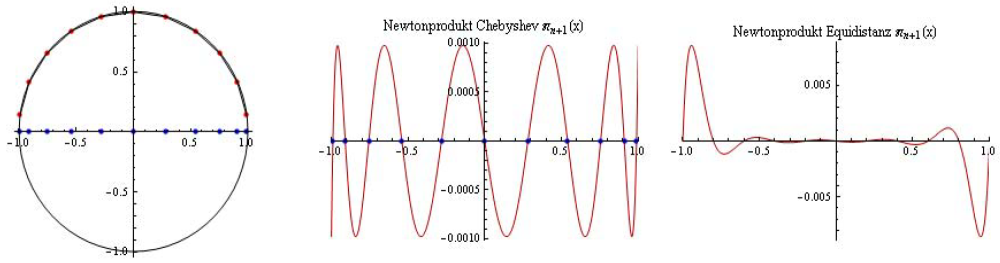
\includegraphics[width=14cm]{bilder/TschbyNewtonVergleich.png}
\end{center}

\textbf{Properties}
\begin{liste}
  \item[+] No Runge Phenomenon (oscillations at the edge)
  \item[+] A single formula
  \item[-] "Not embedded" (new measurements mean new polynomial calculation!)
  \item[-] Practically: Measurements are often only uniformly possible (limited edge resolution)
  \item[-] The range of interpolation is fixed (poor extrapolation outside the edge)
\end{liste}


\subsection{Uniformly Distributed Arguments}

\begin{minipage}[c]{11.0cm}
	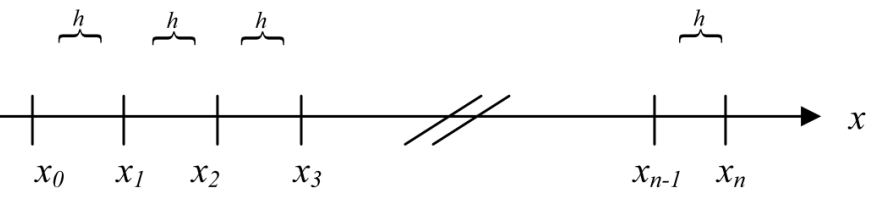
\includegraphics[width=0.8\textwidth]{bilder/gleichvArgum.png}
\end{minipage}
\begin{minipage}[c]{6.0cm}
	$$x_k=x_0+k h\qquad k=0,1,2,\ldots n$$
	$$\boxed{y(x_0,x_1,\ldots,x_k)=\frac{\Delta^k y_0}{h^k k!}}$$
\end{minipage}
\hfill\\

$$p(x)=y_0+\frac{\Delta^1 y_0}{h^1 1!}\pi_1(x)+\frac{\Delta^2 y_0}{h^2 2!}\pi_2(x)+\ldots+\frac{\Delta^n y_0}{h^n n!}\pi_n(x)=\sum\limits_{k=0}^{n}{\frac{\Delta^k y_0}{h^k k!}\pi_k(x)}$$

\begin{center}
    \begin{tabular}{|l|lccccccccc|}
        \hline
        $\Delta^0$ && $y_0$ && $y_1$ && $y_2$ && $y_3$ && $y_4$ \\ \hline
        $\Delta^1$ &&   & $y_1-y_0$ && $y_2-y_1$ && $y_3-y_2$ && $y_4-y_3$ & \\
                   &&   & $\Delta y_0$ && $\Delta y_1$ && $\Delta y_2$ && $\Delta y_3$ & \\ \hline
        $\Delta^2$ && && $\Delta y_1-\Delta y_0$ && $\Delta y_2-\Delta y_1$ && $\Delta y_3-\Delta y_2$ && \\
                   && && $\Delta^2 y_0$ && $\Delta^2 y_1$ && $\Delta^2 y_2$ && \\ \hline
    \end{tabular}
\end{center}


\subsection{Taylor Series}
$$f(x)=\underset{\text{Taylor Polynom p(x)}}{\underbrace{y_0+\frac{y'(x_0)}{1!}(x-x_0)+\frac{y''(x_0)}{2!}(x-x_0)^2+\ldots+\frac{y^{(n)}(x_0)}{n!}(x-x_0)^n}}+\underset{\text{Lagrange Fehlerterm}}{\underbrace{\frac{y^{(n+1)}(\xi)}{(n+1)!}(x-x_0)^{n+1}}}$$
